\section{Framework Overview}

\begin{figure}[htp]
  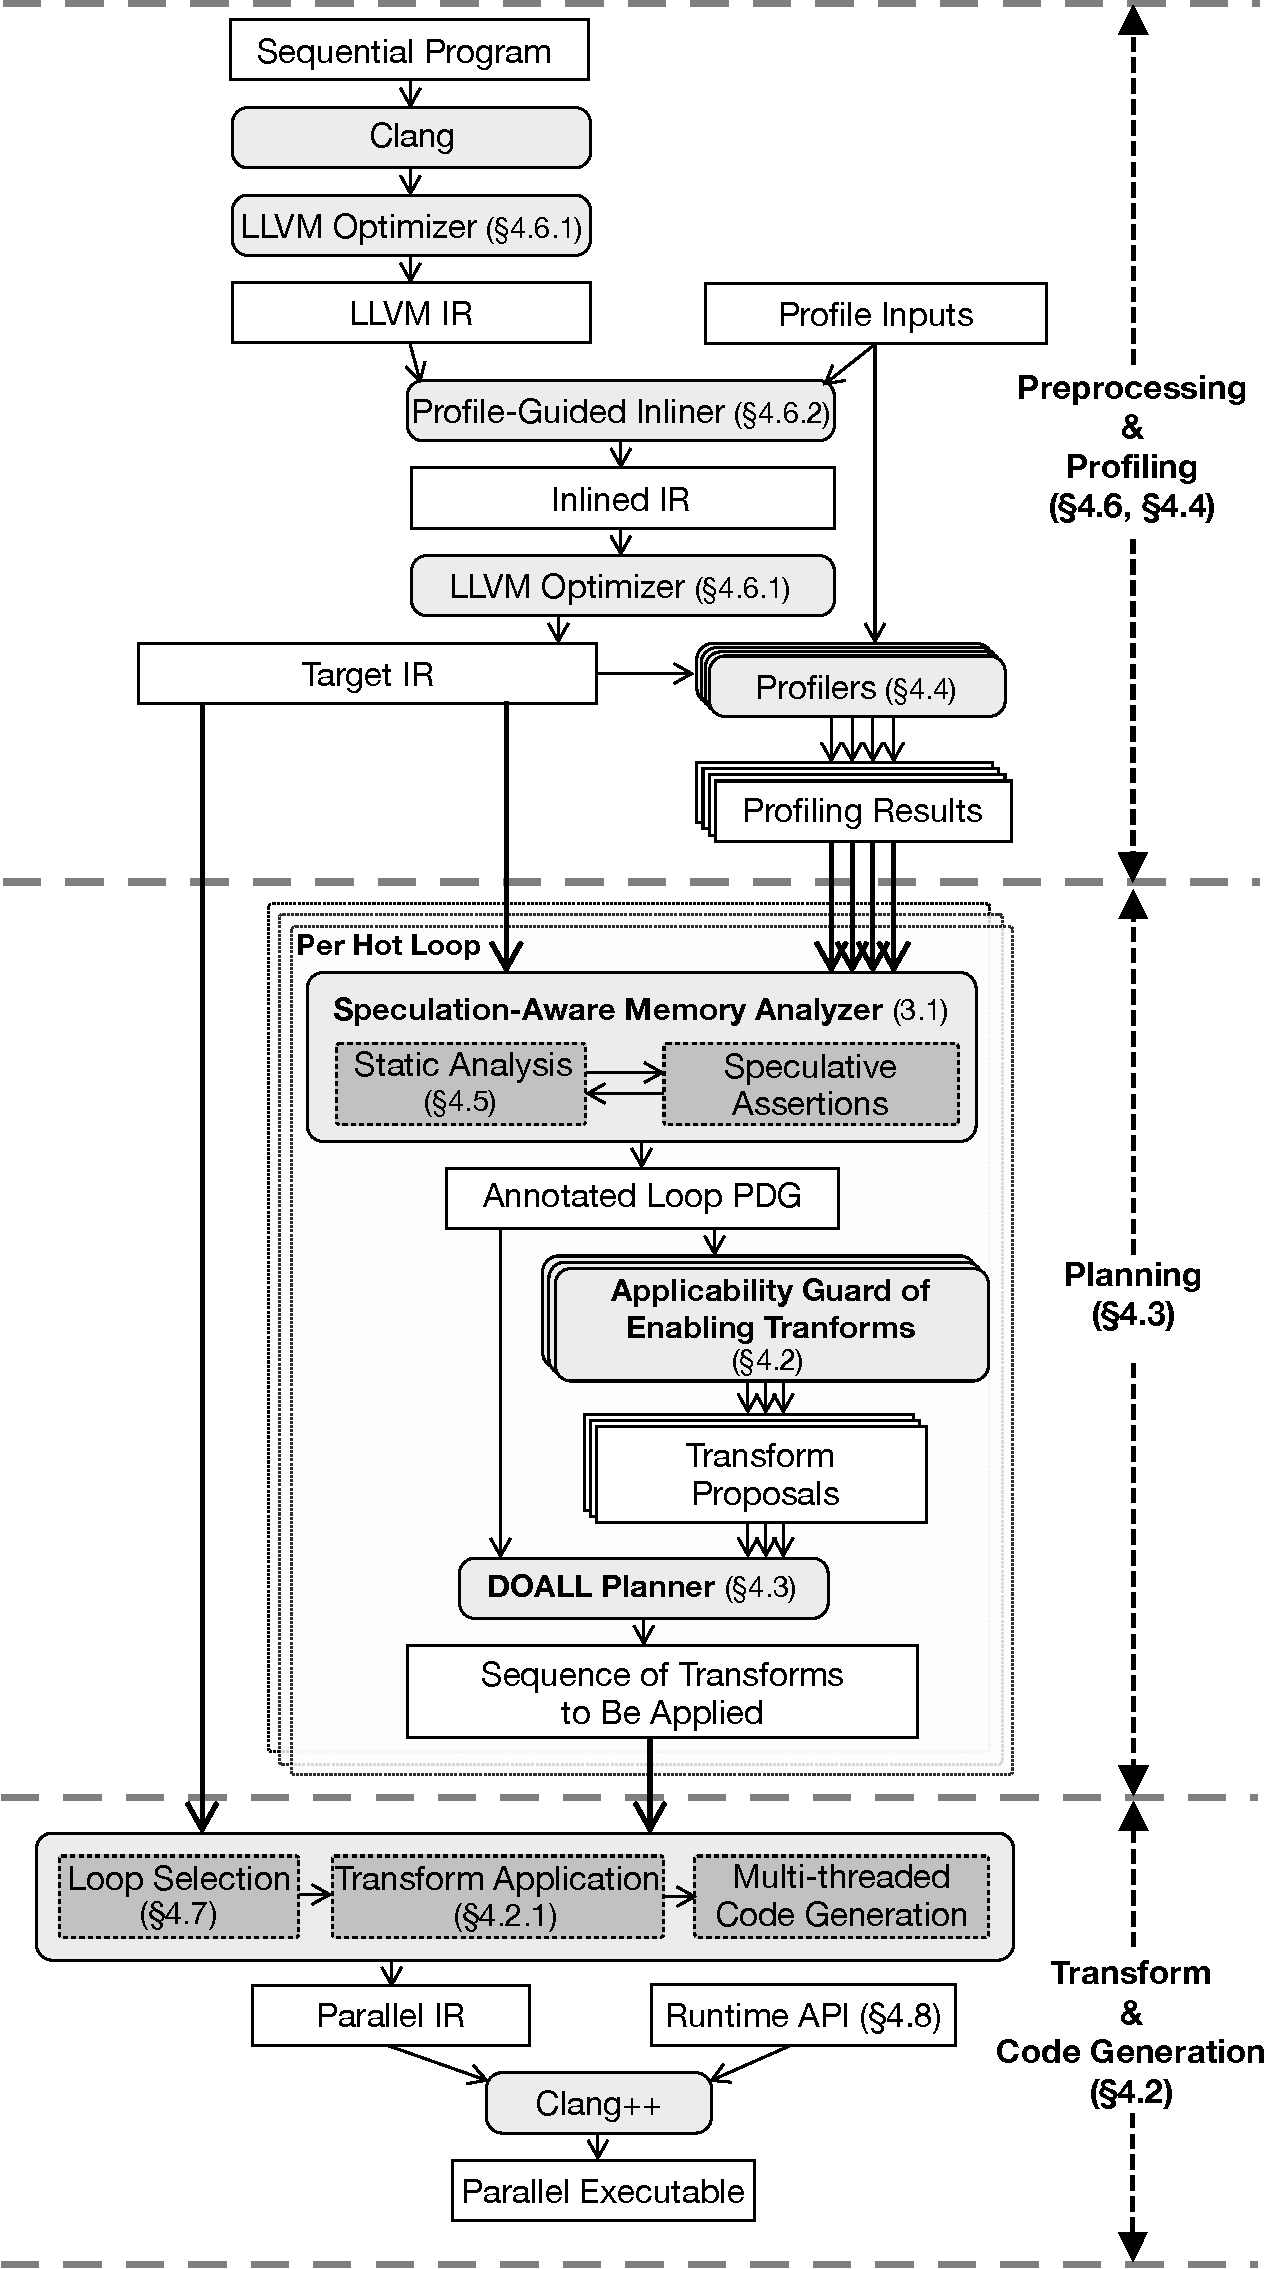
\includegraphics[width=\columnwidth]{figures/compiler-pipeline-crop}
  \caption{Framework Overview}
  \label{fig:compiler-pipeline}
\end{figure}

LSD enables efficient speculative parallelization by leveraging
fine-grained combination of static analysis and cheap-to-validate
assumptions.
%
Figure~\ref{fig:compiler-pipeline} depicts an overview of the LSD system,
which includes a set of profilers, a parallelizing compiler and a runtime
system.
%
The compiler can be split into three regions: Analysis, Planning,
Transformation and Codegen.

We have implemented LSD within the LLVM infrastracture.
Figure~\ref{fig:compiler-pipeline} presents the compiler pipeline of our
framework. As the first step, the sequential program is complied, inlined,
and optimized into a target LLVM intermediate representation (IR) which is
then used to generate profiling results. In the second phase, we focus on
each hot loop, leveraging static and speculative analysis to generate a PDG
annotated with properties of dependences. The analyses for transformations
then examine every remaining loop-carried dependences and propose plans to
remove them. A DOALL planner considers these proposals and generate a
sequence of transformations if a profitable DOALL plan is available.
Finally, we select a set of compatible loops with the maximum profit, apply
tranformations, and generate the parallel IR which is linked with an
efficient uniqued runtime and compiled as the parallel executable.
